\documentclass[a4paper,10pt]{article}
\usepackage[utf8]{inputenc}
\usepackage[italian]{babel}
\usepackage{graphicx}
\usepackage{amsmath}
\usepackage{amssymb}
\usepackage{amsthm}
\usepackage{booktabs}
\usepackage{caption}
\usepackage{geometry}
%\usepackage{hyperref}
\usepackage{makeidx}
\usepackage{microtype}
\usepackage{subfig}
\usepackage{tabularx}
\usepackage{url}
\usepackage{varioref}
\usepackage{xcolor}
\usepackage{multicol}
\usepackage{mathtools}
\usepackage{booktabs}
\usepackage{multirow}
\usepackage{gensymb}
%\graphicspath{ {images/} }
\usepackage{float}
\usepackage{fancyhdr} 
%%%%%%%%%%%%%%%%%%%%%%%%%%%%%%%%%%%%%%%%%%%%%%%%%%%


\title{Laboratorio I: Pendolo fisico\\
\begin{large}
Dipartimento di Fisica E.Fermi - Università di Pisa
\end{large}}

\author{Di Ubaldo Gabriele}
\date{16 Maggio 2016}

\begin{document}
\pagestyle{fancy}
\maketitle
\begin{figure}[!htb]
 \centering
 \includegraphics[width=3cm]{/home/zerch/Documents/UNIPI/Fisica1/images/unipi.jpg}
\end{figure}
\tableofcontents
%%%%%%%%%%%%%%%%%%%%%%%%%%%%%%%%%%%%%%%%%%%%%%%%%%%%%%%%%%%%%%%%%%%%%%%%%%%%%%%%%%%%%%%%%%%%%%%%%%%%%%%%%%%%%%%%%%%%%%%%%%%%%%%%%%%%%%%%%%%%%%%%%%
\section{Introduzione}
\subsection{Teoria}
\textbf{Obiettivo:}Misurare il periodo di un pendolo fisico in funzione della distanza dal centro di massa del punto di sospensione.\\
Ogni oggetto fissato in un punto di sospensione \textbf{P}(polo) spostato di un certo angolo $\phi$ dalla posizione di equilibrio, 
costituisce un pendolo fisico dato che avrà un momento dovuto alla forza di gravità che vale:
\begin{equation}
 \tau=-m g d \sin(\phi)
\end{equation}
che per angoli molto piccoli possiamo approssimare secondo Taylor a $-mgd\phi$.
Impostando la seconda equazione cardinale:
\begin{equation}
\tau=\frac{dL}{dt}
\end{equation}
Otteniamo la seguente funzione $T(d)$:

\begin{equation}
 T(d)=2\pi \sqrt{\frac{(\frac{l^2}{12}+d^2)}{g d}}
\end{equation}

\subsection{Apparato sperimentale}
\begin{figure}[!htb]
 \centering
 \caption{Pendolo fisico}
 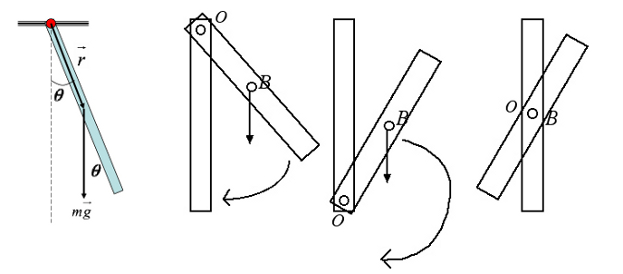
\includegraphics[width=11cm]{/home/zerch/Documents/UNIPI/LAB1/6Penfisico/grafici/penfis.jpg}
\end{figure}

\begin{itemize}
 \item Asta metallica forata
 \item Supporto di sospensione 
 \item Cronometro di risoluzione $0.01s$
 \item Metro a nastro di rissoluzione $1mm$
 \item Calibro ventesimale di risoluzione $0.05mm$
\end{itemize}
%%%%%%%%%%%%%%%%%%%%%%%%%%%%%%%%%%%%%%%%%%%%%%%%%%%%%%%%%%%%%%%%%%%%%%%%%%%%%%%%%%%%%%%%%%
\section{Esperimento}
\subsection{Acquisizione dati}
Posizioniamo l'asta sul supporto e spostando di volta in volta i fori, mettiamo l'asta in oscillazione, sempre con un angolo piccolo e misuriamo di conseguenza il periodo di 10 oscillazioni. Questa procedura è stata ripetuta per 10 fori. per poi fare la media di tutte queste e in seguito dividendo di un fattore 10, al fine di ricavare
il periodo medio in un determinato punto fisso di oscillazione.  
Il pendolo è lungo $l=(1.049 \pm 0.001)m$.
Tutte le misure di periodi, essendo delle misure dirette, posseggono il medesimo errore, equivalente alla risoluzione
dello strumento.

\subsection{Misure}


\begin{table}[!htb]
\centering
\caption{Foro 1}
\label{my-label}
\begin{tabular}{|l|l|l|l|l|l|l|l|l|l|l|}
\hline
             & T1    & T2    & T3    & T4    & T5    & T6    & T7    & T8    & T9    & T10   \\ \hline
Periodo (s)  & 16.41 & 16.33 & 16.24 & 16.22 & 16.34 & 16.33 & 16.34 & 16.32 & 16.29 & 16.33 \\ \hline
Distanza (m) & \multicolumn{10}{l|}{0.474+-0.001}                                             \\ \hline
\end{tabular}
\end{table}
\begin{table}[H]
\centering
\caption{Foro 2}
\label{my-label}
\begin{tabular}{|l|l|l|l|l|l|l|l|l|l|l|}
\hline
             & T1    & T2    & T3    & T4    & T5    & T6    & T7    & T8    & T9    & T10   \\ \hline
Periodo (s)  & 15.73 & 15.59 & 15.69 & 15.59 & 15.74 & 15.64 & 15.61 & 15.60 & 15.57 & 15.61 \\ \hline
Distanza (m) & \multicolumn{10}{l|}{0.374+-0.001}                                             \\ \hline
\end{tabular}
\end{table}
\begin{table}[H]
\centering
\caption{Foro 3}
\label{my-label}
\begin{tabular}{|l|l|l|l|l|l|l|l|l|l|l|}
\hline
             & T1    & T2    & T3    & T4    & T5    & T6    & T7    & T8    & T9    & T10   \\ \hline
Periodo (s)  & 15.66 & 15.48 & 15.49 & 15.60 & 15.61 & 15.65 & 15.63 & 15.59 & 15.60 & 15.58 \\ \hline
Distanza (m) & \multicolumn{10}{l|}{0.274+-0.001}                                             \\ \hline
\end{tabular}
\end{table}
\begin{table}[H]
\centering
\caption{Foro 4}
\label{my-label}
\begin{tabular}{|l|l|l|l|l|l|l|l|l|l|l|}
\hline
             & T1    & T2    & T3    & T4    & T5    & T6    & T7    & T8    & T9    & T10   \\ \hline
Periodo (s)  & 16.76 & 16.72 & 16.91 & 16.83 & 16.88 & 16.83 & 16.78 & 16.69 & 16.80 & 16.69 \\ \hline
Distanza (m) & \multicolumn{10}{l|}{0.174+-0.001}                                             \\ \hline
\end{tabular}
\end{table}
\begin{table}[H]
\centering
\caption{Foro 5}
\label{my-label}
\begin{tabular}{|l|l|l|l|l|l|l|l|l|l|l|}
\hline
             & T1    & T2    & T3    & T4    & T5    & T6    & T7    & T8    & T9    & T10   \\ \hline
Periodo (s)  & 22.60 & 22.90 & 22.08 & 22.78 & 22.67 & 22.68 & 22.71 & 22.83 & 22.77 & 22.83 \\ \hline
Distanza (m) & \multicolumn{10}{l|}{0.073+-0.001}                                             \\ \hline
\end{tabular}
\end{table}
\begin{table}[H]
\centering
\caption{Foro 6}
\label{my-label}
\begin{tabular}{|l|l|l|l|l|l|l|l|l|l|l|}
\hline
             & T1    & T2    & T3    & T4    & T5    & T6    & T7    & T8    & T9    & T10   \\ \hline
Periodo (s)  & 37.89 & 37.87 & 38.07 & 38.17 & 38.19 & 38.17 & 38.02 & 38.15 & 38.12 & 37.92 \\ \hline
Distanza (m) & \multicolumn{10}{l|}{0.024+-0.001}                                             \\ \hline
\end{tabular}
\end{table}
Fino al foro 6, le misure dei periodi sono state prese da una estremità dell'asta avvicinandosi al centro di massa, in seguito
le restanti misure sono state prese ccapovolgendo l'asta, però partendo dal centro di massa fino all'estremità dell'asta.\\
\begin{table}[H]
\centering
\caption{Foro 7}
\label{my-label}
\begin{tabular}{|l|l|l|l|l|l|l|l|l|l|l|}
\hline
             & T1    & T2    & T3    & T4    & T5    & T6    & T7    & T8    & T9    & T10   \\ \hline
Periodo (s)  & 18.53 & 18.58 & 18.57 & 18.53 & 18.40 & 18.51 & 18.42 & 18.53 & 18.53 & 18.56 \\ \hline
Distanza (m) & \multicolumn{10}{l|}{0.124+-0.001}                                             \\ \hline
\end{tabular}
\end{table}
\begin{table}[H]
\centering
\caption{Foro 8}
\label{my-label}
\begin{tabular}{|l|l|l|l|l|l|l|l|l|l|l|}
\hline
             & T1    & T2    & T3    & T4    & T5    & T6    & T7    & T8    & T9    & T10   \\ \hline
Periodo (s)  & 15.90 & 16.01 & 15.97 & 15.95 & 15.97 & 15.96 & 15.91 & 15.99 & 15.90 & 16.00 \\ \hline
Distanza (m) & \multicolumn{10}{l|}{0.224+-0.001}                                             \\ \hline
\end{tabular}
\end{table}
\begin{table}[H]
\centering
\caption{Foro 9}
\label{my-label}
\begin{tabular}{|l|l|l|l|l|l|l|l|l|l|l|}
\hline
             & T1    & T2    & T3    & T4    & T5    & T6    & T7    & T8    & T9    & T10   \\ \hline
Periodo (s)  & 15.75 & 15.71 & 15.74 & 15.62 & 15.63 & 15.67 & 15.75 & 15.65 & 15.69 & 15.57 \\ \hline
Distanza (m) & \multicolumn{10}{l|}{0.324+-0.001}                                             \\ \hline
\end{tabular}
\end{table}
\begin{table}[H]
\centering
\caption{Foro 10}
\label{my-label}
\begin{tabular}{|l|l|l|l|l|l|l|l|l|l|l|}
\hline
             & T1    & T2    & T3    & T4    & T5    & T6    & T7    & T8    & T9    & T10   \\ \hline
Periodo (s)  & 16.04 & 16.00 & 16.01 & 16.09 & 16.07 & 16.10 & 16.03 & 16.08 & 16.09 & 16.01 \\ \hline
Distanza (m) & \multicolumn{10}{l|}{0.424+-0.001}                                             \\ \hline
\end{tabular}
\end{table}
\section{Analisi dati}
Prese le misure, ora andiamo a calcolare media e la deviazione standard sulla media dei periodi e in seguito andremo a confrontare il valore
atteso con quello osservato.
Per calcolare la media, la deviazione standard, e la deviazione standard sulla media utilizziamo:
\begin{equation}
 T_{medio}=\frac{1}{N}\sum_{i=1}^{N}T_i
\end{equation}
\begin{equation}
 \sigma_m=\sqrt{\frac{1}{N-1}\sum_{i=1}^{N}(T_i-{\tilde T_i})^2}
\end{equation}
 \begin{equation}
\sigma_{media}=\frac{\sigma_m}{\sqrt N}
 \end{equation}

Sono state calcolate usando un programma in Python con le funzioni scipy.mean(), numpy.std(ddof=1), scipy.stats.sem() delle rispettive librerie.
Per propagare l'errore sono state usate le solite formule derivante di somma in quadraturaa derivanti dall'espansione di Taylor e la distribuzione gaussiana.

\begin{table}[H]
\centering
\caption{Media e deviazione standard sulla media}
\label{my-label}
\begin{tabular}{|l|l|l|l|l|l|l|l|l|l|l|}
\hline
          & Foro 1 & Foro 2 & Foro 3 & Foro 4 & Foro 5 & Foro 6 & Foro 7 & Foro 8 & Foro 9 & Foro 10 \\ \hline
$T_m$\      & 1.63  & 1.56  & 1.56  & 1.68  & 2.27  & 3.81  & 1.85  & 1.59  & 1.57  & 1.60   \\ \hline
$\sigma_{media}$\ &  0.002 &0.002 &0.002& 0.002& 0.007& 0.004 &0.002& 0.001& 0.002& 0.001 \\ \hline \end{tabular}
\end{table}
\subsection{Fit ed elaborazione dati}
Andiamo ora a tracciare un grafico del periodo in funzione della distanza \textit{d} dal centro di massa, cercando di verificare
l'accordo fra il modello teorico ed i dati sperimentali. Abbiammo posto $g$ come parametro libero per potere valutare l'esito del nostro esperimento anche in base all'accordo col valore noto per Pisa di $g=9.807 m/s^2$.

\begin{figure}[H]
 \centering
 \caption{Grafico del periodo in funzione della distanza}
 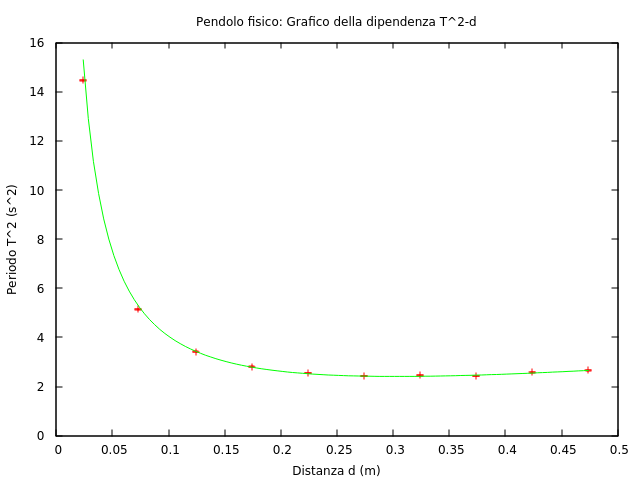
\includegraphics[width=11cm]{/home/zerch/Documents/UNIPI/LAB1/6Penfisico/grafici/graf-t2-1.png}
\end{figure}

I risultati del fit con 9 gradi di libertà sono i seguenti:

\begin{equation}
\chi^2=1010.2 \quad \chi^2_r=112.2 \quad g=9.91\pm0.06 m/s^2 (0.64\%)
\end{equation}

Il $\chi^2 $ assume un valore troppo alto per confermare la validità del nostro modello, nonostante dal grafico si possa osservare un'accordo abbastanza buono tra la curva e i nostri dati. Infatti la probabilità $P(\chi^2<\chi^2_0)\approx 100\%$ Questo può stare ad indicare che abbiamo sottostimato l'errore nelle nostre misure e/o che vi è un errore sistematico.
Il grafico dei residui ci può aiutare a distinguere se vi è un errore sistematico o solo una sottostima dell'errore:

\begin{figure}[H]
 \centering
 \caption{Grafico del periodo in funzione della distanza}
 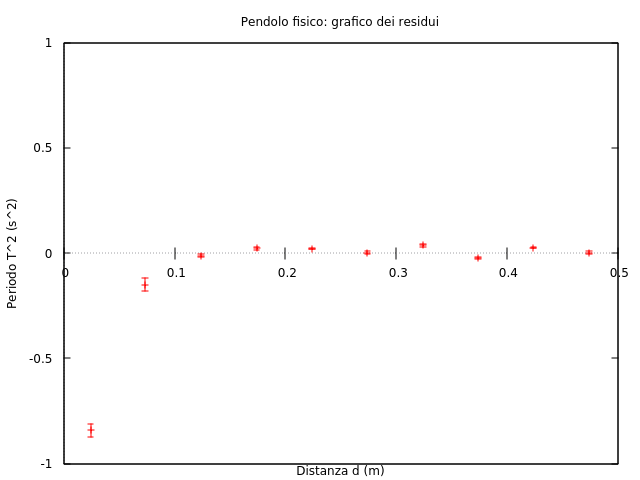
\includegraphics[width=11cm]{/home/zerch/Documents/UNIPI/LAB1/6Penfisico/grafici/residui.png}
\end{figure}

Le prime due misure si discostano molto dal centro e sono quelle che contribuiscono maggiormente al $\chi^2$, questo perchè in quel intorno della funzione $T^2$ la derivata assume valori molto alti rendendo difficile una misura precisa. Per il resto i residui hanno un andamento che porssiamo considerare casuale intorno allo $0$. Possiamo quindi considerare le misure come gaussiane ed eliminare la possibilità che vi sia stato un errore sistematico in una direzione o nell'altra. 
Considerando l'errore invece che al millisecondo, al centesimo di secondo possiamo vedere dal seguente grafico che vi è un accordo notevolmente migliore tra la teoria e i dati sperimentali.
\begin{figure}[H]
 \centering
 \caption{Grafico del periodo in funzione della distanza}
 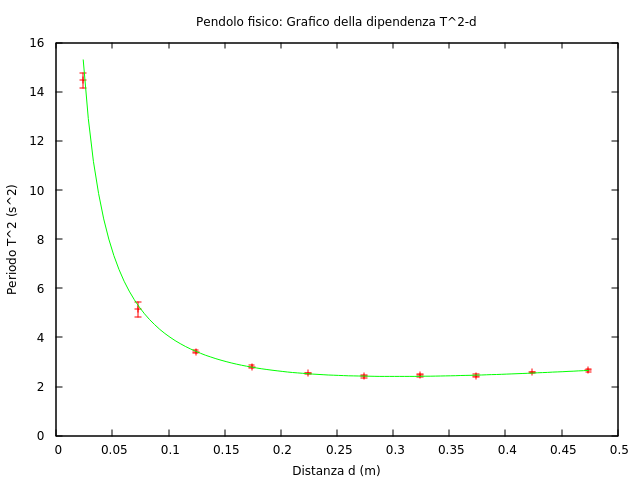
\includegraphics[width=11cm]{/home/zerch/Documents/UNIPI/LAB1/6Penfisico/grafici/graf-t2-2.png}
\end{figure}

I risultati del fit con 9 gradi di libertà sono i seguenti:

\begin{equation}
\chi^2=10.1 \quad \chi^2_r=1.12 \quad g=9.91\pm0.06 m/s^2 (0.64\%)
\end{equation}
Il $\chi^2$ è molto vicino al numero di gradi di libertà: il valore che ci aspetteremmo dalla distribuzione di probabilità del $\chi^2$ è $\chi=9\pm\sqrt{18}=9\pm4.24$ quindi il nostro valore è definitivamente compatibile e soddisfacente, il che ci permette di confermare l'accordo della teoria con le misure effettuate. 
Il valore di $g$ ottenuto è compatibile entro $2\sigma$ dal valore noto il che è un'altra conferma della validità del nostro esperimento.
La probabilità $P(\chi^2<\chi^2_0)=65.7\%$ rientra nella convenzione del $95\%-5\%$.
Molto probabilmente la fonte di errore trascurata è l'imprecisione umana nell'uso del cronometro considerando che non è possibile misurare con una precisione tale che l'errore sia dell'ordine del millisecondo. È molto più realistico e corretto considerare il nostro errore di un ordine di grandezza maggiore.

Il grafico dei residui con l'errore ristimato è il seguente:

\begin{figure}[H]
 \centering
 \caption{Grafico dei residui dopo analisi dell'errore}
 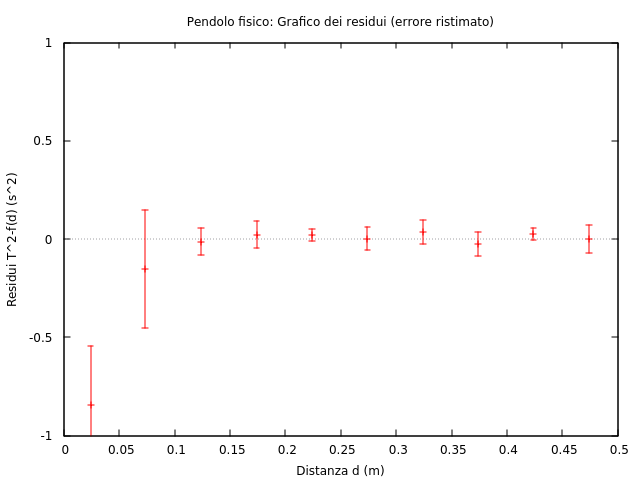
\includegraphics[width=11cm]{/home/zerch/Documents/UNIPI/LAB1/6Penfisico/grafici/residui2.png}
\end{figure}

Come possiamo vedere ora la maggior parte delle misure non si discosta più di un $\sigma$ dal valore dato dal fit.


\section{Conclusioni}
Possiamo concludere affermando che l'errore sulle misure era stato sottostimato, per tale motivo il test del  $\chi^2$ non confermava la validità del modello. Dopo aver analizzato l'errore e le sue cause lo abbiamo corretto e abbiamo ottenuto un sostanziale accordo tra teoria ed esperimento.
L'esperimento può dirsi concluso in successo con una stima di $g$ come:
\begin{equation}
g=9.91\pm 0.12 (2\sigma) m/s^2
\end{equation}
\end{document}
